% Design Requirements
\chapter{Appendices - Characteristics of Embraer jet E175}

\section{Analysis of aircraft dimensions}
\textbf{Dimensions for the seats:}
Here are the characteristic dimensions of the seats of an Embraer jet E175 in economy class:
\begin{figure}[h]
\centering
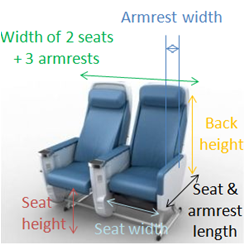
\includegraphics[width=7cm]{images/seat_dimensions_image_global.png}
\caption{Seats of a typical Embraer E175 in economy class}
\label{fig:seat_dimensions_1}
\end{figure}

\begin{figure}[h]
\centering
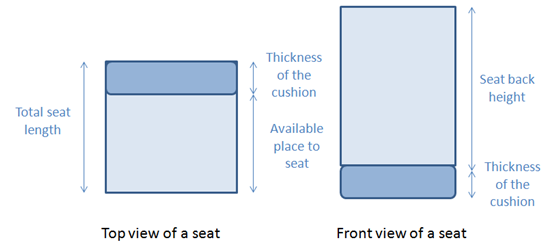
\includegraphics[width=7cm]{images/seat_dimensions_image_topandfront_view.png}
\caption{Characteristics of the seat}
\label{fig: seat_dimensions_2}
\end{figure}

\begin{figure}[h]
\centering
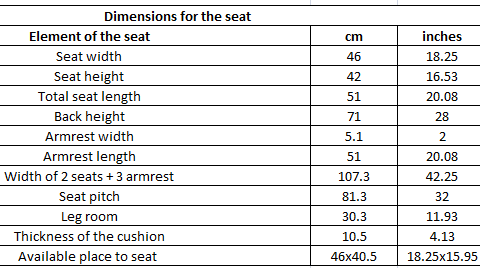
\includegraphics[width=7cm]{images/seat_dimensions_table}
\caption{Table presenting all of the dimensions that define an airplane seat}
\label{fig: seat_dimensions_table}
\end{figure}

\textbf{Dimensions of the fuselage:}
In order to determine what are the constraints of our design space we wanted to have a precise map of the aircraft fuselage and its available space for passengers. Here are the characteristic dimensions of the fuselage of an Embraer jet E175.
\begin{figure}[h]
\centering
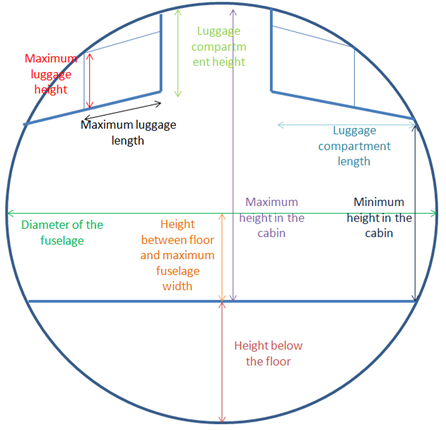
\includegraphics[width=7cm]{images/fuselage_dimensions}
\caption{Characteristic dimensions of the fuselage of an Embraer jet E175}
\label{fig: fuselage_dimensions}
\end{figure}

\begin{figure}[h]
\centering
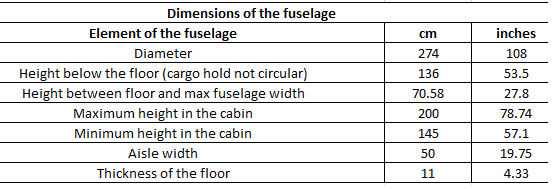
\includegraphics[width=7cm]{images/fuselage_table}
\caption{Table presenting all of the dimensions of the fuselage of an Embraer jet E175}
\label{fig:fuselage_table}
\end{figure}

\textbf{Dimensions of the luggage compartment inside the cabin:}
To take advantage of the available space inside the cabin our team wanted to analyze the volume and the space dedicated to carry-on luggage. All of the dimensions of the luggage compartment are represented on \ref{fig:fuselage_table} and their values are presented in \ref{fig:luggage_compartment_table}.
\begin{figure}[h]
\centering
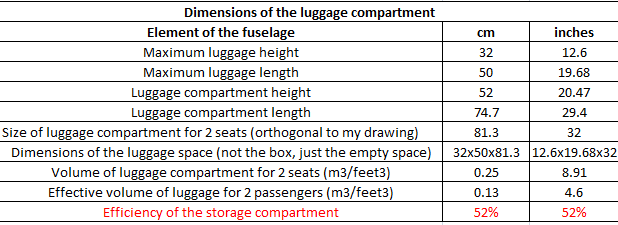
\includegraphics[width=7cm]{images/luggage_compartment_table.png}
\caption{Table presenting all the dimensions of the fuselage of an Embraer jet E175}
\label{fig:luggage_compartment_table}
\end{figure}

From the previous analysis we noticed that only 52\% of the luggage compartment is actually dedicated to carry-on storage. This is because the remaining 48\% are dedicated to wires, light and air conditioned systems.

\section{Analysis of the cargo hold structure}

\textbf{Characteristics of the material used for the cargo hold floor}
In order to protect the passengers’ wheelchairs from damages, our team decided to design a structure that would enclose the wheelchair while stored in the cargo hold. In order to understand what are the constraints the will have to deal with during our design process we decided to analyze both the geometric and structural constraints caused by the aircraft structure.
\\
\textbf{Geometric constraints due the cargo hold shape:}

On \ref{fig:aircraft_structure} we can see that the geometry of the cargo hold is an important limitation for our design since the semi elliptical shape considerably reduces the volume and height available for storage.

\begin{figure}[h]
\centering
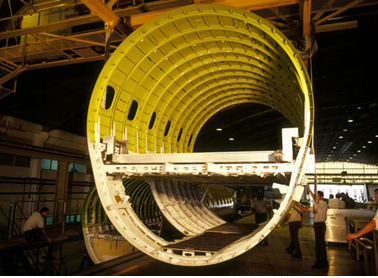
\includegraphics[width=7cm]{images/aircraft_structure.png}
\caption{Structure of an Embraer jet E170 \cite{embraer_struct}}
\label{fig:aircraft_structure}
\end{figure}

In order to make sure that the product we want to design to protect the wheelchair is adapted to the cargo hold dimensions we looked at two elements:

\begin{easylist}[itemize]

& The cargo hold characteristic dimensions that are shown on \ref{fig:cargo_hold_geometry_table} 

\begin{figure}[h]
\centering
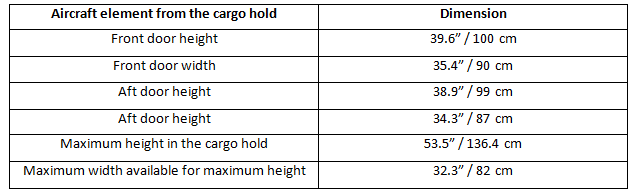
\includegraphics[width=7cm]{images/cargo_hold_geometry_table.png}
\caption{Cargo hold characteristic dimensions}
\label{fig:cargo_hold_geometry_table}
\end{figure}

& The characteristic dimensions of one of the biggest powered wheelchair that is available on the market (\ref{fig:heavy_wheelchair}). Its dimensions are shown on \ref{fig:wheelchair_geometry_table}.

\begin{figure}[h]
\centering
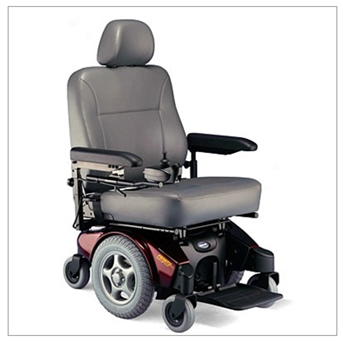
\includegraphics[width=7cm]{images/heavy_wheelchair.png}
\caption{One of the heaviest powered wheelchair of the market designed for obese disabled people (https://www.shermanoaksmedical.com/M94\_p/m94-invacare.htm)}
\label{fig:heavy_wheelchair}
\end{figure}

\begin{figure}[h]
\centering
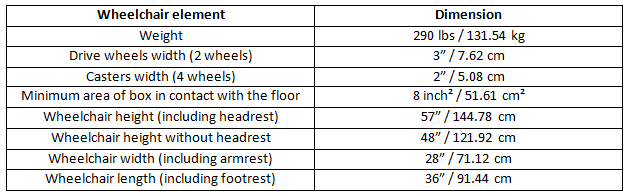
\includegraphics[width=7cm]{images/wheelchair_geometry_table.png}
\caption{Table presenting all the dimensions of the wheelchair}
\label{fig:wheelchair_geometry_table}
\end{figure}

\end{easylist}

By comparing the wheelchair dimensions to the cargo hold dimensions, we noticed that the headrest has to be remove otherwise the wheelchair is too high to fit the cargo hold. Fortunately, most of the heavy powered wheelchairs are equipped with removable parts in order to minimize the size and weight of the wheelchair while this latter is transported from one place to another.

One the headrest is removed this wheelchair can be stored in the cargo hold. Its width is lower than the doors’ width so it can enter the cargo hold. Even if the height of the wheelchair is higher than the cargo hold door’s height, by tilting the wheelchair airline employees are able to make it go inside the cargo hold.

To conclude about the geometric constraints of the cargo hold, given that the biggest wheelchairs can be stored inside the cargo hold of an Embraer jet, the only restriction we really need to take into account is the clearance between the product we will design to protect the structure and the size of the door. For instance, if we decide to use inflatable material to protect the wheelchair, we may have to blow it up inside the cargo hold and not outside in order to make sure the package size will still be smaller than the door size.

\textbf{Structural constraints due the cargo hold structure:}

As previously mentioned when our team interviewed the Air France employee in charge of cargo hold management, wheelchairs can be very heavy and the contact area with the cargo floor is very small. This can generate stress that the cargo hold floor will not be able to withstand. In order to design a product that will protect the wheelchair inside the cargo hold, our team needed to analyze the stress limitations of the cargo hold floor to take them into account in our design process.

Hexcel is a US company that provides aircraft manufacturers with composite material (beams and panels) used in the cargo hold floor structure. On their website (www.hexcel.com) we were able to get the technical data sheet of Fiberlam, the material that is used for the cargo hold structure of Embraer jet C-28-1386 Type II MEP 15-031.

From these data, here are the calculations made to determine the maximum pounds per square inch the cargo hold floor can withstand. Knowing that there are different types of elements below the floor, we calculated the maximum load for each type of beam and its main failure mode and chose the most sensitive value as our limitation.
On \ref{fig: types_beam_cargo_hold} we can see the three different types of beam that constitute the cargo hold structure:
\begin{easylist}
& The long beams that come across the entire fuselage. Because they are very long they are very sensitive to bending and flexural failure.
& The short beams that are very close to the fuselage skin and are designed to withstand traction and compression force. They are not very resistant to shear forces since they are not suppose to experience them a lot.
& The floor panels that are sensitive to flatwise compression.
\end{easylist}{itemize}
\begin{figure}[h]
\centering
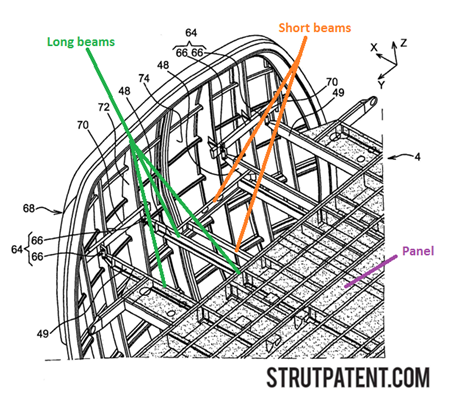
\includegraphics[width=7cm]{images/types_beam_cargo_hold}
\caption{Different types of elements that constitute the cargo hold structure from http://www.strutpatent.com/patent/07338013/floor-for-aircraft}
\label{fig: types_beam_cargo_hold}
\end{figure}

The average skin stress can be determined with the following equation:
Skin stress : \[ \sigma_{s} = \frac{P.s}{8.(h-t).wt} \]
\begin{figure}[h]
\centering
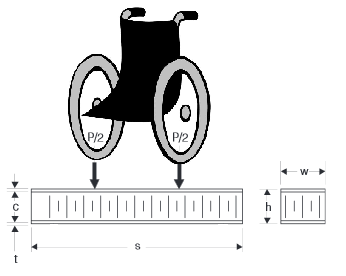
\includegraphics[width=7cm]{images/structural_analysis}
\caption{Key parameters for the structural analysis of the cargo hold floor stress}
\label{fig: structural_analysis}
\end{figure}
\\
s = beam span (2489 inches / 980 cm) \\
P = total applied load on the surface of the beam (distributed or punctual) \\
t = skin thickness (0.015 inches / 0.038 cm) \\
w = width of panel (24.4 inches / 9.6 cm) \\
h = panel thickness (0.66 inches / 1.7 cm) \\

For $ P_{max}$ = 490 lbs or 2170 N which is a typical value for the rupture of a sandwich panel being used as aircraft floor, the maximum skin stress we can tolerate is $ \sigma_{s}$= 6222 psi or 42.9 MPa.
This is associated with a maximum stress of $Stress_{max 1}$ = 6222 psi or 42.9 MPa.
\subsubsection{Analysis of short beams – shear failure}
For such a beam, the typical failure mode is a shear failure in the core of the beam (not the skin). Provided that the failure occurs in the core, the core shear strength (average shear stress) can be calculated by the following equation:
Shear stress: \[ \tau = \frac{P}{2.c.w} \]
\\
P = total load applied on the surface of the beam (distributed or punctual)\\
c = core thickness (0.645 inches / 1.662 cm)\\
w = width of panel (30.48 inches / 12 cm)\\

For $P_{max}$ = 710 lbs or 3150 N which is a typical value for the rupture of the core of a sandwich panel being used as aircraft floor, the maximum applied load we can tolerate is $ \tau$ = 36.11 psi or 0.25MPa.
This is associated with a maximum stress of $Stress_{max 2}$ = 36.11 psi or 0.25 MPa on the beam. This value is quite low because these beams are designed to withstand mainly traction and compression forces. They are poor in shear resistance.
\subsubsection{Analysis of floor panels – flat wise tension/compression failure}
We want to determine the core compressive limitation of the sandwich panel. Since we have a sandwich panel with thin face skin, the following equation can be used to determine the strength of the core:
\[ \sigma = \frac{P}{s.w} \]
with s = 144 inches / 365.8 cm and w = 32.3 inches / 82 cm \\
$ \sigma =$ 740 psi or 5.1 MPa is a typical value for the rupture of a sandwich panel being used as aircraft floor. This is directly associated with a maximum stress of $ Stress_{max 3} =$ 740 psi or 5.1 MPa on the floor.

In conclusion, the most sensitive parts of the cargo hold floor are the short beams:
$Stress_{max 2} < Stress_{max 3} < Stress_{max 1}$
 This is because these beams are designed to reinforce the cargo hold structure when it is in tension due to pressurization. Since these beam are design to withstand tension loads if a very heavy element of the cargo hold applies a shear force on them they are quite sensitive to it and do not resist it very well contrary to the floor panels and long beams which are specifically designed for this.
As a consequence, we need to design our wheelchair protection system such that the distributed load applied on the cargo hold floor does not exceed $ Stress_{max 2} =$ 36.11 psi or 0.25 MPa. It means that for a wheelchair such as \ref{fig:heavy_wheelchair} we need to distribute the load over a minimum contact area with the floor which is 8 $inches^2$ – 51.61 $cm^2$. The ‘floor’ of our protection system must exceed this surface.



